\documentclass[pdflatex,sn-mathphys-num]{sn-jnl}

\usepackage{graphicx}
\usepackage{amsmath,amssymb,amsfonts}
\usepackage{booktabs}

\raggedbottom

\begin{document}

\title[Empirical limits of k-sighted decision trees]{One split at a time is often enough: empirical limits of k-sighted decision-tree induction}

\author*[1]{\fnm{Mathias} \sur{Valla}}

\affil*[1]{\orgname{Affiliation to be completed}, \orgaddress{\country{France}}}

\abstract{Decision trees are usually induced by greedy recursive splitting, although a split's value depends on the subtree it permits. A k-sighted tree is a natural intermediate between greedy induction and exact optimal-tree search: it preserves the recursive tree-growing paradigm but scores candidate splits through a bounded descendant subtree. We study whether this additional non-greedy optimization materially improves shallow decision trees and random forests when predictive accuracy and fitting time are evaluated jointly. On a sample of 67 PMLB classification datasets, integer sight depths $k=2$ and $k=3$ raised observed mean accuracy over ordinary $k=1$ greedy induction, but only by small and uneven margins. For single trees, mean accuracy increased from 0.6931 to 0.7100 and 0.7145, while mean fitting time increased from 0.008 s to 0.373 s and 70.90 s. For forests, mean accuracy increased from 0.7068 to 0.7125 and 0.7260, while fitting time increased from 0.019 s to 0.694 s and 96.19 s. A simple accuracy-time utility calculation makes the tradeoff explicit: over the tested depths, modest accuracy gains were accompanied by orders-of-magnitude increases in fitting time. Mixed forests with a small fraction of farther-sighted trees are then used to ask whether a few expensive trees can raise mean accuracy in a mostly greedy ensemble. These descriptive results suggest that k-sighted induction is better viewed as a targeted tool than as a default replacement for greedy CART-style induction.}

\keywords{Decision trees, Random forests, K-sighted trees, Greedy algorithms, Optimal trees, PMLB}

\maketitle

\section{Introduction}\label{sec:introduction}

The standard decision-tree algorithm makes a sequence of local decisions. At each internal node it selects the split that most improves an impurity criterion, then repeats the same operation on the two child nodes \cite{quinlan1986induction,breiman1984cart}. This strategy is fast, simple, and effective enough to remain the foundation of single decision trees, bagged trees, and random forests \cite{breiman1996bagging,breiman2001random}. Its weakness is equally clear: a split is not useful in isolation, but because of the subtree it enables. A locally weak split may create children that are easy to separate, while a locally strong split may make subsequent separation difficult.

This paper studies the practical value of relaxing that greediness. A k-sighted tree scores a candidate split by looking $k$ generations ahead, choosing the split whose best bounded descendant subtree gives the largest impurity reduction. The method is appealing because it occupies a middle ground: it is less myopic than CART-style induction, but far less ambitious than exact global optimization of the whole tree.

The research question is deliberately narrow: does bounded multi-step split optimization deliver enough predictive accuracy to justify its computational cost? We answer this question empirically for shallow single trees and forests under a fixed screening protocol. The central finding is that larger $k$ can raise mean accuracy, but the gain is small and uneven compared with the increase in fitting time. The result is not that greedy trees are optimal; they are not. It is that greedy induction remains highly competitive once time is part of the objective.

\section{Related work}\label{sec:related}

Top-down induction of decision trees was codified in ID3, CART, and related algorithms as a greedy search over split scores or impurity reductions \cite{quinlan1986induction,breiman1984cart}. Bagging and random forests changed the statistical behavior of greedy trees by averaging many unstable predictors \cite{breiman1996bagging,breiman2001random}, but they did not remove the greedy split-selection mechanism inside each tree. This matters for the present study because extra sight inside a forest competes not only with a single greedy tree, but also with the error-reduction effect of ensembling.

Multi-step tree induction has a long history. Norton \cite{norton1989generating} proposed generating better decision trees by considering downstream tree quality, and Ragavan and Rendell \cite{ragavan1993lookahead} studied descendant-aware feature construction for difficult concepts. Murthy and Salzberg \cite{murthy1995lookahead} gave a particularly relevant warning: adding one extra generation of split search can be much more expensive and does not reliably improve accuracy, a phenomenon they connected to pathology in decision-tree induction. Elomaa and Malinen \cite{elomaa2005lookahead} further analyzed multi-step split search and pathology. Esmeir and Markovitch \cite{esmeir2007anytime} reframed tree induction as an anytime process, where additional computation should be justified by measurable improvement in the learned tree. Our work follows this cost-sensitive perspective.

At the other end of the spectrum, exact or near-exact optimal-tree methods search directly over tree structures. Hyafil and Rivest \cite{hyafil1976constructing} showed that constructing optimal binary decision trees is NP-complete. Modern mixed-integer and branch-and-bound approaches have made optimal trees practical in selected regimes \cite{bertsimas2017optimal,verwer2019learning,hu2019optimal,lin2020generalized,aghaei2025strong}, but scalability remains central. Other non-greedy methods optimize tree parameters jointly or through surrogate objectives \cite{norouzi2015efficient}. K-sighted induction is therefore an intermediate case: it asks whether a small amount of structured non-greediness captures enough of the available gain to be worthwhile in routine induction.

\section{K-sighted induction and an accuracy-time utility}\label{sec:method}

Let $S$ be the samples reaching a node, let $I(S)$ be the node impurity, and let $\mathcal{T}_k(s,S)$ denote the frontier leaves obtained after applying candidate split $s$ at the current node and then recursively choosing descendant splits for at most $k-1$ additional generations. A k-sighted split maximizes
\begin{equation}
G_k(s;S) =
I(S) -
\sum_{L \in \mathcal{T}_k(s,S)}
\frac{|L|}{|S|} I(L).
\label{eq:sighted}
\end{equation}
Sight depth $k=1$ is ordinary greedy induction. Depths $k=2$ and $k=3$ choose a split using the best two- or three-generation bounded subtree available under the same candidate-split mechanism.

Increasing $k$ changes the local training-set criterion from immediate impurity decrease to impurity after a bounded descendant expansion. This can correct a myopic split, but it need not improve held-out accuracy or preserve the greedy ranking of root splits. The difficulty is computation. If $m$ candidate splits are considered at each internal node, the number of split configurations in a full binary k-sighted subtree has a naive upper bound of order $m^{2^k-1}$. Practical implementations reuse work and stop at pure or infeasible nodes, but the qualitative pressure remains: sight depth increases the search cost much faster than it increases the number of fitted tree levels.

To compare accuracy with time, we use a simple descriptive utility heuristic. Suppose mean predictive accuracy and mean fitting time at sight depth $k$ are approximated by
\begin{equation}
A(k) \approx A(1) + \alpha(k-1),
\qquad
T(k) \approx T(1)\exp\{\beta(k-1)\}.
\end{equation}
For a user who values accuracy but penalizes multiplicative increases in fitting time, define
\begin{equation}
U_\lambda(k) = A(k) - \lambda \log\left(\frac{T(k)}{T(1)}\right),
\label{eq:utility}
\end{equation}
where $\lambda$ is the accuracy cost assigned to one natural-log unit of additional time. Relative to the greedy baseline, a larger sight depth has higher utility only if
\begin{equation}
A(k)-A(1) > \lambda \log\left(\frac{T(k)}{T(1)}\right).
\end{equation}
Thus the empirical quantity
\[
\lambda^\star_k =
\frac{A(k)-A(1)}{\log(T(k)/T(1))}
\]
is a break-even value: if the chosen time penalty exceeds $\lambda^\star_k$, greedy induction has higher utility under this model. The calculation is not intended as a full decision-theoretic model; it is a compact way to put accuracy and fitting time on the same scale.

\section{Experiments}\label{sec:experiments}

We evaluated sight depths $k \in \{1,2,3\}$ for a decision-tree classifier and a random-forest classifier on a sample of 67 PMLB classification datasets \cite{olson2017pmlb}. The experimental protocol was fixed throughout: a single train-test split, stratified when possible, test size $0.25$, random state $0$, maximum tree depth $3$, all features available at each split, and no explicit cap on split candidates. The forest experiments used 100 bootstrap trees with the same k-sighted rule inside each tree, so the comparison isolates the split-selection rule rather than feature subsampling.

We recorded test accuracy and wall-clock fitting time. Wall-clock times are implementation- and hardware-dependent, but their order of magnitude is relevant because larger $k$ changes the fitting problem itself. The goal is not to prove that extra sight never helps. Rather, it is to measure, under this fixed benchmark setting, whether a routine move from one-step to multi-step split optimization changes the practical accuracy-cost frontier for shallow trees and forests.

For forests, mixtures of integer sight depths provide an additional way to spend computation. If a forest contains proportions $p_j$ of trees with integer sight depths $k_j$, we summarize the mixture by its effective sight depth
\[
\bar{k}=\sum_j p_j k_j .
\]
This scalar is a useful shorthand rather than a complete description: a forest with 90\% $k=1$ trees and 10\% $k=2$ trees has $\bar{k}=1.10$, as does a forest with 95\% $k=1$ trees and 5\% $k=3$ trees, although the latter spends its extra computation differently. We used this construction to test whether a small number of farther-sighted trees can raise mean accuracy in a mostly greedy ensemble.

\section{Results}\label{sec:results}

Table~\ref{tab:aggregate} summarizes the main benchmark. Mean accuracy is higher at larger $k$ in both model families, but the gain is modest compared with the cost. For single trees, $k=2$ raises mean accuracy by 1.69 percentage points over $k=1$, while mean fitting time is about 49 times larger. The $k=3$ tree raises mean accuracy by 2.15 percentage points, while mean fitting time is about $9.4\times 10^3$ times larger. For forests, $k=2$ raises mean accuracy by 0.57 percentage points, while mean fitting time is about 37 times larger. The $k=3$ forest raises mean accuracy by 1.92 percentage points, while mean fitting time is about $5.1\times 10^3$ times larger.

\begin{table}[t]
\caption{Aggregate performance over 67 PMLB classification datasets.}
\label{tab:aggregate}
\begin{tabular}{@{}lrrrr@{}}
\toprule
Estimator & Sight depth & Mean accuracy & Median accuracy & Mean fit time (s)\\
\midrule
Decision tree & 1 & 0.6931 & 0.7554 & 0.0076\\
Decision tree & 2 & 0.7100 & 0.7222 & 0.3727\\
Decision tree & 3 & 0.7145 & 0.7333 & 70.9025\\
Random forest & 1 & 0.7068 & 0.7500 & 0.0188\\
Random forest & 2 & 0.7125 & 0.7407 & 0.6940\\
Random forest & 3 & 0.7260 & 0.7612 & 96.1864\\
\botrule
\end{tabular}
\end{table}

Figure~\ref{fig:accuracy_time} displays the empirical pattern. Accuracy gains remain modest over the three sight depths, while fitting time grows by orders of magnitude on the same grid, consistent with the exponential-time side of the heuristic above. This mismatch is the central empirical result: the k-sighted signal is visible in the mean, but the computational price rises much more sharply.

\begin{figure}[t]
\centering
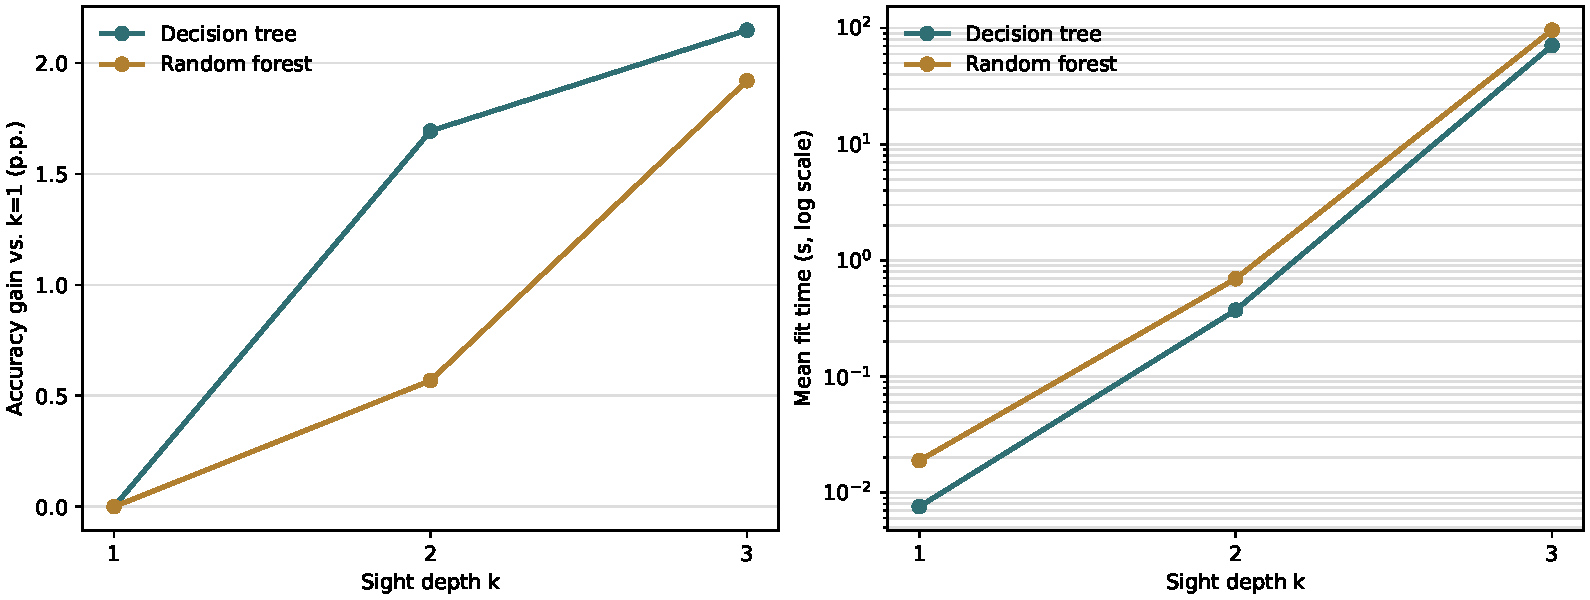
\includegraphics[width=\textwidth]{Fig1_accuracy_time.pdf}
\caption{Mean accuracy gain and mean fitting time as sight depth increases from $k=1$ to $k=3$. Accuracy gains are measured relative to the greedy $k=1$ baseline. Fitting time is shown on a logarithmic scale.}
\label{fig:accuracy_time}
\end{figure}

The utility heuristic in Eq.~\eqref{eq:utility} makes the tradeoff explicit. The break-even values $\lambda^\star_k$ are 0.00435 for tree $k=2$ versus $k=1$, 0.00235 for tree $k=3$ versus $k=1$, 0.00158 for forest $k=2$ versus $k=1$, and 0.00225 for forest $k=3$ versus $k=1$. These values correspond to roughly 0.16--0.44 percentage points of accuracy per natural-log unit of additional fitting time. Under this heuristic, any larger penalty for training-time growth would favor the greedy baseline in these aggregate comparisons.

The gains are also not uniform. Counting ties as wins, so that more than one depth may be credited on the same dataset, $k=1$ was tied for the best single-tree accuracy on 30 datasets, $k=2$ on 31 datasets, and $k=3$ on 37 datasets. For forests, the corresponding counts were 36, 29, and 29. The median results reinforce the same point: $k=2$ has a higher mean than $k=1$ in both model families, but a lower median accuracy. Larger $k$ therefore changes the average, but it does not dominate the greedy rule across datasets.

\subsection{Can a few farther-sighted trees help a forest?}\label{subsec:forestsize}

We next asked whether extra sight should be concentrated in a few trees rather than applied to the whole ensemble. Figure~\ref{fig:forest_size} compares integer $k \in \{1,2,3\}$ forests across several forest sizes on the completed smaller-dataset mixed-forest sample ($n=57$) and adds 100-tree mixed forests: 95/5, 90/10, 75/25, and 50/50 mixtures of $k=1$ and $k=2$ trees, a 95/5 mixture of $k=1$ and $k=3$ trees, and a 95/5 mixture of $k=2$ and $k=3$ trees. These mixtures ask whether a small farther-sighted minority can raise mean accuracy for the whole forest.

\begin{figure}[t]
\centering
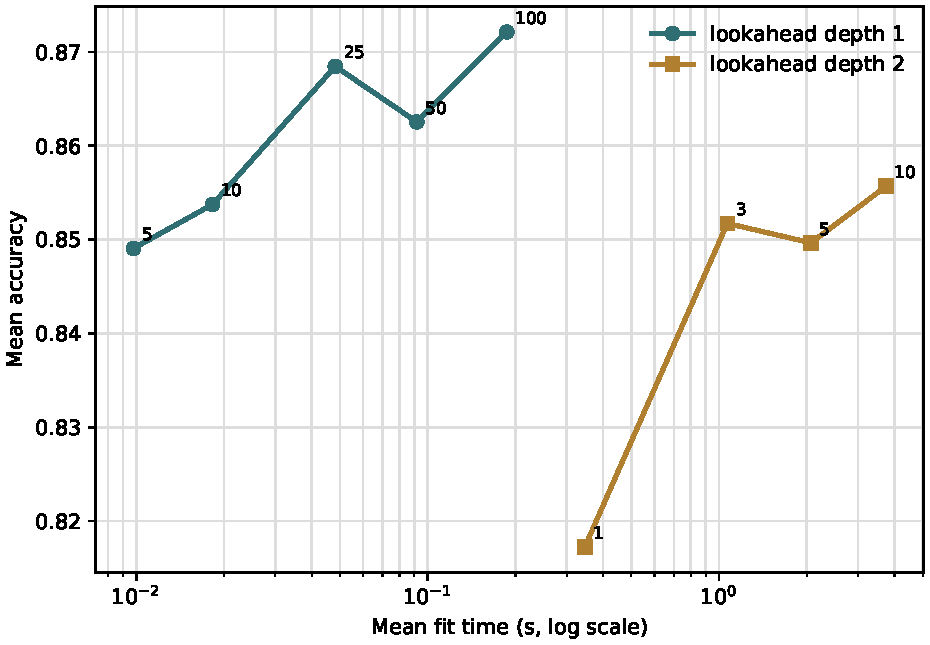
\includegraphics[width=0.75\textwidth]{Fig2_forest_size.pdf}
\caption{Forest size, integer sight depth, and mixed k-sighted forests over the completed smaller-dataset mixed-forest sample ($n=57$). Line labels indicate the number of trees in pure integer-depth forests. Diamond markers are 100-tree mixtures; the label 1.10 appears twice because 90\% $k=1$ plus 10\% $k=2$ and 95\% $k=1$ plus 5\% $k=3$ have the same effective sight depth but different computational profiles.}
\label{fig:forest_size}
\end{figure}

The mixed-forest frontier is more informative than a yes-or-no answer. On this sample, a 100-tree greedy forest reached 0.7229 mean accuracy in 0.211 s. Replacing 5\%, 10\%, 25\%, and 50\% of the trees by $k=2$ trees increased mean accuracy to 0.7286, 0.7336, 0.7428, and 0.7478, while increasing mean fit time by factors of 2.6, 4.1, 8.9, and 16.7. A fully $k=2$ 100-tree forest reached 0.7513 accuracy at 32.5 times the greedy fit time. Thus a small $k=2$ minority can raise mean accuracy, but it behaves like a gradual accuracy-time tradeoff rather than a disproportionate ensemble-level effect. The $k=3$ mixtures are less attractive in this experiment: a 95\% $k=1$ plus 5\% $k=3$ forest had almost the same accuracy as the 95/5 $k=1$/$k=2$ mixture, but took about 121 times the greedy fit time. Adding 5\% $k=3$ trees to a mostly $k=2$ forest barely changed mean accuracy relative to the pure $k=2$ forest and roughly quadrupled the fit time.

\section{Discussion}\label{sec:discussion}

The empirical result is clear but limited: k-sighted induction is a plausible correction to greedy myopia, but it is not a compelling default under this protocol. The benchmark shows that larger $k$ can raise mean accuracy. Yet the improvement is thin relative to the cost, and it is not consistent across datasets.

This conclusion helps explain the durability of greedy decision trees. Greedy splitting is not merely a historical convenience; it gives a strong accuracy-time compromise. Random forests further reduce the cost of myopic split decisions by averaging many greedy trees. Once this ensemble mechanism is available, spending large amounts of computation inside each split decision has to clear a high bar. Mixed k-sighted forests sharpen the same point: a few expensive trees may help on average in this sample, but they must compete with the cheap variance reduction obtained by simply adding greedy trees.

The utility model is intentionally simple, but useful. When accuracy gains remain incremental while time grows by orders of magnitude, the marginal utility of larger $k$ must eventually collapse for any positive time penalty. This does not rule out k-sighted induction. It identifies where it may be most useful: small problems, shallow trees, specialized interaction structures, interpretability settings where a single stronger tree is valuable, or cases where computation is cheap relative to the cost of prediction errors. The present evidence should be read with the same restraint: the protocol uses shallow trees, a fixed train-test split, and mean accuracy-time summaries rather than a full model-selection study.

\section{Conclusion}\label{sec:conclusion}

Multi-step split optimization can raise measured accuracy for decision trees and random forests, but in these experiments it does so by a narrow margin and at a very large computational cost. The practical lesson is therefore conservative. Greedy CART-style induction is not globally optimal, but it remains a remarkably strong default. For routine shallow tabular trees and forests, one split at a time is often the better starting point.

\backmatter

\bmhead{Data availability}
The benchmark datasets are available from PMLB \cite{olson2017pmlb}. Aggregate tables, plotting scripts, and the implementation used for this study are included in the accompanying repository branch.

\bmhead{Code availability}
The k-sighted tree implementation and manuscript-generation scripts are included in the accompanying repository branch.

\bmhead{Funding}
Funding information is to be completed before submission.

\bmhead{Competing interests}
The author declares no competing interests.

\bibliography{references}

\end{document}
